\documentclass[leqno,10pt]{article}
\usepackage{algorithm}
\usepackage{array}
\usepackage[noend]{algpseudocode}
\usepackage{hyperref}
\usepackage[linewidth=1pt]{mdframed}
\usepackage{float}
\def\Z{\mathbb Z}
\def\Q{\mathbb{Q}}
\def\A{\mathbb{A}}

\makeatletter
\renewcommand{\ALG@name}{Algorytm}
\makeatother

\usepackage{amsmath}
\usepackage{float}
\usepackage{delta}
\usepackage{todonotes}
\usepackage{authblk}

\newcommand{\edge}{\mbox{\rotatebox[origin=c]{90}{\ddagger}}\xspace} 

\def\marg#1{\marginpar{\scriptsize\raggedright#1}}

\usepackage{delta}
\def\marg#1{\marginpar{\scriptsize\raggedright#1}}
\usepackage[normalem]{ulem}
\newcounter{nchng}\renewcommand{\thenchng}{\stepcounter{nchng}(\bf\color{blue}\arabic{nchng})}
\newcommand{\note}[1]{
\let\thefootnote\relax\footnote{\color{blue}\ensuremath{^{(\bf\color{blue}\arabic{nchng})}}#1}}
\newcommand{\nnote}[1]{{\color{blue}\textrm{\ensuremath{^{\thenchng}}}}
\let\thefootnote\relax\footnote{\color{blue}\ensuremath{ ^{(\bf\color{blue}\arabic{nchng})} }#1}}
\newcommand{\add}[1]{{\color{blue}#1\ensuremath{^{\thenchng} }}}
\newcommand{\remove}[1]{{\color{red}\sout{#1}}\textrm{\ensuremath{^{\thenchng} }}}
\newcommand{\change}[2]{{{\color{red}\sout{#1}}\color{blue}#2\ensuremath{^{\thenchng} }}}
\renewcommand{\note}[1]{}\renewcommand{\add}[1]{#1}
\renewcommand{\remove}[1]{}\renewcommand{\change}[2]{#2}
\renewcommand{\nnote}[1]{}
\begin{document}

\wtyt{O pewnym modelu zawijania białek}


\waut{Marcin WIERZBIŃSKI$^{1,2}$, Karolina L. TKACZUK$^{2}$, Alessandro CRIMI$^{2}$}


\marg{[1] Student, Wydział Matematyki, Informatyki i Mechaniki, Uniwersytet Warszawski, [2] Sano Centrum Medycyny Obliczeniowej w Krakowie}

Aminokwasy to małe cząsteczki stanowiące główny budulec białka. 
Można o nich myśleć jak o koralikach nawleczonych na sznurek, a sposób ich ułożenia w przestrzeni
decyduje o funkcji białka w komórce oraz o tym, jak oddziałuje ono z innymi
elementami komórki. Z tego względu struktura przestrzenna danego białka jest dla
badaczy bardzo pożądaną informacją m.in. w przypadku projektowania leków.

Istnieje wiele możliwości odtworzenia kształtu białka występującego w naturze.
Jedną z bardziej standardowych jest ,,hodowla'' cząsteczki w warunkach
laboratoryjnych, imitujących te naturalne. 
Jest to metoda bardzo czasochłonna i nie zawsze skuteczna, gdyż uchwycenie białka
nie zawsze bywa możliwe -- białko może okazać się niestabilne i rozpaść się przed odtworzeniem jego
kształtu.
Alternatywą dla tej metody jest tworzenie trójwymiarowych struktur ,,w krzemie'' (tj. przy
użyciu komputera) w oparciu o modele teoretyczne. Podstawą tych ostatnich są
istniejące już struktury białek (wcześniej odtworzone eksperymentalnie i zebrane
w bazie białek \href{www.rcsb.org}{\textit{Protein Data Bank}}). W
ostatnich latach temat zyskał duże zainteresowanie mediów, ze względu na sukcesy
projektu AlphaFold
(\href{https://alphafold.ebi.ac.uk}{alphafold.ebi.ac.uk}), który do
przewidywania struktur białek wykorzystuje sztuczną inteligencję.

Jednym z najprostszych modeli
struktury przestrzennej białek jest model hydrofobowo-polarny (HP), 
w którym aminokwasy podzielone są na dwa typy: $H$
(aminokwas hydrofobowy) i $P$ (aminokwas hydrofilowy). Białko jest w nim
reprezentowane przez zagięcie danej skończonej sekwencji $s \in\{H, P\}^{k}$ w
kracie $L=\mathbb{Z}^{3}$.
\textit{Zagięcie} (lub \textit{zwinięcie}) możemy formalnie zdefiniować jako przekształcenie różnowartościowe $\omega:\{1,\ldots,k\} \rightarrow L$, takie że sąsiednie liczby odpowiadają sąsiednim
punktom z kraty, tzn.
\begin{equation*}
		 \omega(i) \neq \omega(j)
		 \quad\textrm{oraz}\quad
		 |\omega(i)-\omega(i+1)|=1
		 \quad\textrm{dla }
     1 \leq i<j \leq k, 
\end{equation*}
przy czym $|p-q|$ to zwyczajna (euklidesowa) odległość między punktami
$p$ i $q$.
Poszukiwane jest zagięcie o największej liczbie $P$ par sąsiadujących w kracie aminokwasów typu
$H$. Wartość $-P$ określa się w tym kontekście mianem \textit{energii}; innymi
słowy, szukamy zatem zagięcia o najmniejszej energii.

\marg{\vspace*{-3cm}
\begin{center}
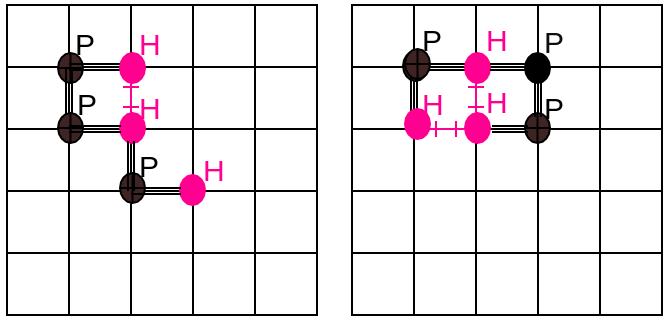
\includegraphics[width=4.8cm]{diagram3.png}
\end{center}
Przykłady zagięcia sekwencji $s={HPPHPH}$ w kracie $\mathbb{Z}^{2}$. Po
lewej stronie energia całkowita jest równa $-1$, a po prawej stronie $-2$.
Co więcej, zagięcie przedstawione po prawej stronie realizuje globalne minimum energii
całkowitej. 
}

Dla krótkich sekwencji aminokwasów (tzn. niewielkich wartości $k$) optymalne
zagięcie można odnaleźć, obliczając energię każdego możliwego zagięcia. W
praktyce jednak długości sekwencji mogą mieć od $50$ do ponad $1500$ aminokwasów, a
liczba możliwych zagięć rośnie bardzo szybko wraz ze wzrostem $k$! 
W umieszczonej na marginesie tabeli przedstawiono liczbę zagięć w kracie $\Z^3$ dla wybranych
wartości $k$; jasno wynika z niej, że przeszukiwanie wszystkich konfiguracji nie
wchodzi w grę.
\marg{
\begin{center}
\begin{tabular}{c|c}
$k$   &  liczba zagięć w $\Z^3$\\
\hline
1  & 6 \\
2  & 30 \\ 
3  & 150 \\
4  & 726 \\
5  & 3534 \\
10 & $\sim 8{,}8\cdot 10^6$ \\
15 & $\sim 21{,}2\cdot 10^9$  \\
20 & $\sim 49{,}9 \cdot 10^{12}$ \\
\end{tabular}
\end{center}
}
\marg{O przybliżaniu liczby możliwych zagięć metodami Monte Carlo można przeczytać w artykule Wojciecha Niemiro \textit{Monte Carlo, spacery i
polimery} w $\Delta_{15}^5$.}

To, że przestrzeń możliwości jest ogromna nie oznacza jeszcze, że z
informatycznego punktu widzenia problem jest nie do rozwiązania. Przyjrzyjmy się
bliżej trudności naszego zadania.
Sformułowany przez nas problem ma charakter obliczeniowy -- szukamy zagięcia $\omega$
minimalizującego energię zadaną pewnym wzorem. To zdanie może zostać
przeformułowane następujący w problem decyzyjny (nazwijmy go $ZB$ --
\textit{Zwijanie Białka}). 

\begin{mdframed}
\textbf{Wejście}: Ustalona sekwencja $s \in \{H,P\}^{k}$, liczbę naturalna $m \in \mathbb{N}$.

\textbf{Pytanie:} Czy istnieje zawinięcie sekwencji $s \in \{H,P\}^{k}$ w kracie $
\mathbb{Z}^3$ o energii co najmniej $-m$? 
\end{mdframed}

Gdybyśmy znali szybki algorytm rozwiązujący $ZB$, moglibyśmy
uruchamiać go dla coraz większych wartości $m$, by uzyskać informacje o
minimalnej energii zagięcia. Okazuje się jednak, że nasze decyzyjne zadanie jest
problemem NP-zupełnym, czyli z punktu widzenia informatyka w ścisłym sensie
bardzo trudnym (o takich problemach można przeczytać np. w
$\Delta^{01}_{17}$ oraz $\Delta^{11}_{17}$). 

NP-zupełność problemu zagięć białek
została wykazana w artykule \textit{Protein Folding in the Hydrohobic-Hydorphilic HP
Model is NP-Complete} autorstwa Bonniego Bergera i Toma Leightona. 
% Artykuł jest miejscami dość techniczny, jednak autorzy postarali się dostarczyć
% pewnych intuicji stojących za ich rozumowaniem.
Schemat tego (miejscami mocno skomplikowanego) dowodu jest następujący: zamiast
problemu $ZB$ rozważają oni problem $WS$ (\textit{Wypełnianie Sześcianu}):
\begin{mdframed}
\textbf{Wejście}: Liczba naturalna $n$ i ustalona sekwencja $s \in \{H,P\}^{k}$, w której znajduje się
$n^3$ liter $H$.

\textbf{Pytanie:} Czy istnieje zawinięcie sekwencji $s \in \{H,P\}^{k}$ w kracie $
\mathbb{Z}^3$, w którym litery $H$ wypełniają sześcian $n\times n\times n$? 
\end{mdframed}

Jest dość intuicyjne, że umiejętność rozwiązania problemu $ZB$ pociąga za sobą
zdolność do rozwikłania $WS$; wystarczy wziąć $m=3n^2(n-1)$, czyli tyle ile jest
krawędzi w sześciennej siatce $n\times n\times n$. Nietrudno bowiem uwierzyć, że
sześcienna siatka jest najbardziej optymalnym rozwiązaniem z punktu widzenia
liczby sąsiadujących liter $H$. Następnie dowodzi się, że problem $WS$ jest tak
samo trudny, jak poniższa wersja \textit{problemu pakowania plecaka}, o
której wiadomo że jest $NP$-trudna.

\begin{mdframed}
\textbf{Wejście}: 
Liczby naturalne $B$ i $K$, zbiór $U$ oraz funkcja $s\colon U\to
\mathbb{N}$ przyjmująca wartości parzyste, taka że $\sum_{u\in U} s(u)=BK$

\textbf{Pytanie:} Czy można podzielić zbiór $U$ na $K$ podzbiorów $U_i$
($i=1,\ldots,K$) w taki sposób, że dla każdego $i$ mamy $\sum_{u\in U_i}
s(u)=B$?
\end{mdframed}

Wiemy już, że zadanie znajdowania optymalnego zwinięcia jest problemem trudnym.
Czy to oznacza, że jesteśmy skazani na wybieranie ,,na ślepo'' losowych zwinięć i
wskazywanie spośród nich tego o najmniejszej energii, choć wiemy że w ten sposób
przeglądamy tylko malutką część całej przestrzeni? Na szczęście nie; można czynić coś istotnie mądrzejszego. Jednym z podejść jest oznaczanie tras,
którymi się już przechodziło i które nie dały interesującego zagięcia. Taki
pomysł stosowany jest w algorytmie \textit{Monte Carlo Tree Search}. Ten algorytm został
wykorzystany m.in. w słynnym programie Alpha Go.
\marg{
W listopadzie $2015$ roku jako
pierwszy automat, Alpha Go pokonał zawodowego gracza w grę Go, Fan Hui,w
pięciorundowym pojedynku na pełnej planszy w równej grze. AlphaGo był początkowo
szkolony na archiwalnych grach, aby naśladować styl gry graczy, wykorzystując
bazę danych zawierającą około $30$ milionów ruchów. 
}

 W naszym przypadku ,,gra'' (jednoosobowa) może być
określona jako wydłużanie zawinięć w taki
sposób, by uzyskać jak najmniejszą energię i skończyć, gdy długość
sekwencji wynosi $k$. 
Monte Carlo Tree Search dla modelu hydrofobowo-polarnego na każdym etapie
działania algorytmu operuje na drzewie dotychczas sprawdzonych ruchów, czyli
zawinięć częściowych. Każde z tych zawinięć ma obliczone dotychczasowe empiryczne
oszacowanie jakości.
Krok algorytmu polega na 
\begin{itemize}
\item wyborze liścia $\mathcal{L}$ aktualnego drzewa: startując od korzenia
(tylko pierwszy aminokwas) wybieramy dzieci kolejnych wierzchołków tak, by maksymalizować pewną
funkcję (zależną od aktualnej jakości wierzchołków i tego, jak często były odwiedzane na
dotychczasowych etapach), aż dojdziemy do liścia drzewa
\item rozszerzeniu zwinięcia $\mathcal{L}$ o kolejny aminokwas z sekwencji w losowym
kierunku i dołączenie tak powstałego zwinięcia $\mathcal{C}$ do aktualnego drzewa.
\item rozszerzaniu $\mathcal{C}$ o kolejne aminokwasy z sekwencji w losowych
kierunkach, aż do otrzymania zwinięcia długości $k$. Powtórzenie tej operacji wielokrotnie i na
tej podstawie wyznaczenie jakości $\mathcal{C}$ jako średniej energii końcowych
zwinięć uzyskanych w symulacji.
\item aktualizacji jakości wierzchołków drzewa na drodze od $\mathcal{C}$ do
korzenia drzewa (na podstawie wcześniejszych symulacji z $\mathcal{C}$).
\end{itemize}
Mam nadzieję, że tym przykładem przekonałem Czytelnika, że algorytmy losowe mają ciekawe zastosowanie praktyczne,
które przydaje się w poszukiwaniu przybliżonych rozwiązań dla określonych
modeli. Sam model hydrofobowo-polarny daje bardzo ciekawe teoretyczne wyniki i
wiąże się on z istotnymi problemami informatyki, statystyki i matematyki.  

\end{document}
